% Post-Quantum Cryptography Migration on Bitcoin — Deployment, Agility & Governance
% Bitcoin Core edition of the BGIN GDC26 breakout deck
% (GDC26_PQC_Migration_DLTs_Slides.pdf, BGIN – Mitchell Travers & Shin'ichiro Matsuo, 3 Sep 2026).
% Same 17-slide structure and look; wording re-angled for the Bitcoin Core and Bitcoin
% infrastructure community; the two diagram slides (9, 10) that rendered blank in the
% original are drawn here. Facts follow bgin-global/pqc-agility-competition (draft v0).
% Build: latexmk -pdf GDC26_PQC_Migration_Bitcoin_Core_Slides.tex
\documentclass[aspectratio=169,10pt]{beamer}
\usepackage[utf8]{inputenc}
\usepackage[T1]{fontenc}
\usepackage{helvet}
\renewcommand{\familydefault}{\sfdefault}
\usepackage{booktabs}
\usepackage{array}
\usepackage{graphicx}
\usepackage{fontawesome5}
\usepackage{tikz}
\usetikzlibrary{arrows.meta,positioning,calc}
\usepackage{qrcode}
\usepackage{hyperref}

% ---------- look: dark title bar, white body, grey footer (as in the original) ----------
\usetheme{default}
\definecolor{bar}{RGB}{25,25,29}
\definecolor{ink}{RGB}{35,35,40}
\definecolor{soft}{RGB}{110,110,118}
\definecolor{boxbg}{RGB}{242,242,244}
\definecolor{lane}{RGB}{225,227,232}
\setbeamercolor{normal text}{fg=ink}
\setbeamercolor{structure}{fg=bar}
\setbeamercolor{frametitle}{bg=bar,fg=white}
\setbeamercolor{block body}{bg=boxbg,fg=ink}
\setbeamertemplate{navigation symbols}{}
\setbeamertemplate{itemize item}{\color{bar}\faAngleRight}
\setbeamertemplate{enumerate item}{\colorbox{bar}{\color{white}\scriptsize\insertenumlabel}}
\setbeamerfont{frametitle}{series=\bfseries,size=\large}
\setbeamertemplate{frametitle}{%
  \vskip-2pt\begin{beamercolorbox}[wd=\paperwidth,ht=8mm,dp=2.5mm,leftskip=6mm]{frametitle}%
  \usebeamerfont{frametitle}\insertframetitle\end{beamercolorbox}}
\setbeamertemplate{footline}{%
  \begin{beamercolorbox}[wd=\paperwidth,ht=5mm,dp=2mm,leftskip=6mm,rightskip=6mm]{normal text}%
  \tiny\color{soft}\raisebox{-1.2pt}{
\includegraphics[height=3.2mm]{bgin_mark.png}}\hspace{1.2mm}%
  BGIN --- PQC Migration on Bitcoin \textperiodcentered{} Bitcoin Core edition\hfill
  October 2026 / \insertframenumber\end{beamercolorbox}}
\newcommand{\takeaway}[1]{\par\vspace{1.5mm}{\small\color{bar}\faLink~\textbf{Takeaway:} #1}}
\newcommand{\lead}[1]{\begin{beamercolorbox}[wd=\textwidth,sep=2.5mm]{block body}\small #1\end{beamercolorbox}\par\vspace{2mm}}
\newcommand{\pillar}[3]{\begin{minipage}[t]{#1}\colorbox{bar}{\parbox{\dimexpr\linewidth-2\fboxsep}{\color{white}\small\textbf{#2}}}\par\vspace{1mm}{\small #3}\end{minipage}}
\hypersetup{colorlinks,urlcolor=bar,linkcolor=ink}

\begin{document}

% ---------------------------------------------------------------- 1 title
{\setbeamertemplate{footline}{}
\begin{frame}[plain,t]
  \begin{tikzpicture}[remember picture,overlay]
    \fill[bar] (current page.north west) rectangle ([yshift=-3.1cm]current page.north east);
    \node[anchor=north east,inner sep=0] at ([xshift=-7mm,yshift=-5mm]current page.north east){
\includegraphics[height=1.9cm]{bgin_logo.png}};
    \node[anchor=west,text=white,font=\Large\bfseries] at ([xshift=7mm,yshift=-1.55cm]current page.north west){Post-Quantum Cryptography Migration on Bitcoin};
    \node[anchor=west,text=white,font=\small,text width=11.2cm,align=left] at ([xshift=7mm,yshift=-2.45cm]current page.north west){Deployment, Agility \& Governance --- a working frame for Bitcoin Core and Bitcoin infrastructure};
    \node[anchor=west,font=\normalsize] at ([xshift=7mm,yshift=-4.5cm]current page.north west){BGIN -- Mitchell Travers \& Shin'ichiro Matsuo};
    \node[anchor=west,font=\small,text=soft] at ([xshift=7mm,yshift=-5.15cm]current page.north west){Bitcoin Core \& Bitcoin infrastructure community \textbar{} October 2026};
    \node[anchor=west,font=\scriptsize,text=soft,text width=13cm,align=left] at ([xshift=7mm,yshift=-6.2cm]current page.north west){Adapted from the BGIN breakout at Global Digital Collaboration, Geneva, 2--3 September 2026 \textperiodcentered{} ecosystem-neutral: no chain and no scheme is endorsed};
  \end{tikzpicture}
\end{frame}}

% ---------------------------------------------------------------- 2 frame
\begin{frame}{Post-Quantum Cryptography Migration on Bitcoin}
  \lead{Bitcoin's UTXO set relies on long-lived cryptographic trust: secp256k1 ECDSA and Schnorr (BIP-340). NIST-standardized post-quantum cryptography is available. The work in this room is \textbf{deployment, crypto agility, and governance} --- not a new algorithm contest, and not a chain endorsement.}
  {\small\textbf{Where this frame comes from}}
  \begin{itemize}\small
    \item The BGIN breakout \emph{PQC Migration on DLTs} at Global Digital Collaboration (Geneva, September 2026). Co-organizers: ISO; Blockchain Group --- BGIN, Blockchain Bundesverband e.V., Ethereum Climate Platform, LNet; Linux Foundation Group --- OpenWallet, Trust Over IP, LF Decentralized Trust.
    \item BGIN's IKP working group, which has carried crypto agility and PQC migration as a standing item since Block 12.
    \item Japan's government-hosted PQC Migration Prize (METI/NEDO), whose evaluation BGIN coordinates --- with Bitcoin as one of the two evidence anchors.
  \end{itemize}
  \takeaway{This deck asks what Bitcoin Core reviewers, wallet and signing-device vendors, custodians and miners each need to see before a migration design can be judged --- and what a neutral testbed must measure to give it to them.}
\end{frame}

% ---------------------------------------------------------------- 3 not another primitive
\begin{frame}{The Job Is Not to Pick Another Primitive}
  \lead{First PQC standards are in place (ML-KEM, ML-DSA, SLH-DSA; FN-DSA in draft). Re-running a competition in this room would waste the hour.}
  {\small What still has no agreed playbook for Bitcoin:}
  \begin{itemize}\small
    \item How to stage a hybrid and then a cutover when validity rules change only by soft fork and every node must agree.
    \item How to keep verifying ECDSA and Schnorr for as long as classical UTXOs remain spendable.
    \item How to move coins whose public keys are already exposed --- P2PK outputs, reused addresses, revealed keys --- without stranding dormant holders or deciding their fate for them.
    \item How to tell a genuine PQ-ready stack from a screenshot.
  \end{itemize}
  \takeaway{Treat PQC as a multi-year systems and governance program, not a weekend library swap.}
\end{frame}

% ---------------------------------------------------------------- 4 not like TLS
\begin{frame}{Why This Stack Does Not Migrate Like TLS}
  \begin{center}\small
  \begin{tabular}{@{}p{6.2cm}p{7.6cm}@{}}\toprule
    \textbf{Enterprise PKI / TLS} & \textbf{Bitcoin}\\ \midrule
    An operator can force a cutover & No single party can force a soft fork; users, miners, node operators and implementations each hold a practical veto\\
    Cipher suites can be negotiated per session & Script validity rules are global and sticky; a new output type needs activation\\
    Certificates expire on a known clock & On-chain signatures must stay verifiable for decades; the UTXO set is the archive\\
    Harvest-now, decrypt-later is mainly archival & Public keys sit in the clear in P2PK outputs, reused addresses and every spend\\
    Evidence lives in a vendor report & ``PQ-ready'' claims need comparable measurement: vbytes per block, validation time, UTXO growth\\ \bottomrule
  \end{tabular}\end{center}
  \takeaway{A TLS playbook fails on three axes at once: decentralized upgrades, long-lived authenticity, and economic incentives.}
\end{frame}

% ---------------------------------------------------------------- 5 two halves
\begin{frame}{Two Halves of the Same Conversation}
  \lead{Migration urgency is a function of resource estimates. Bitcoin rooms keep hearing ``migrate now'' and ``decades away'' from different speakers. This frame holds both halves in one place.}
  \pillar{0.48\textwidth}{Resource estimates}{What would actually be required to break secp256k1 signatures, under which assumptions, and with which honest error bars. The August 2026 PRX Quantum paper from Google Quantum AI et al.\ puts the ECDLP at about 1{,}200 logical qubits and 90M Toffoli gates (or 1{,}450 / 70M) and sorts attacks into on-spend, at-rest and on-setup. No calendar marketing of a single Q-day.}\hfill
  \pillar{0.48\textwidth}{Migration and agility}{Hybrid signatures, staged activation, quantum-resistant output types in the P2QRH / BIP-360 direction (a reference mapping, not an endorsement), wallet and Lightning / L2 impact, post-quantum ZKP where proofs are in the trust path, and MPC where key management takes the hit.}
  \takeaway{The estimates set the clock. The architecture sets whether the clock can be met without a rushed incident.}
\end{frame}

% ---------------------------------------------------------------- 6 exists / gap
\begin{frame}{What Already Exists --- and the Honest Gap}
  \begin{columns}[T]
    \begin{column}{0.48\textwidth}
      {\small\textbf{Already standardized or public}}
      \begin{itemize}\small
        \item NIST PQC primitives: FIPS 204 / 205, FIPS 206 draft, SP 800-208 stateful hash-based
        \item Hybrid patterns in adjacent Internet protocols
        \item Bitcoin proposals in the P2QRH / BIP-360 direction; public resource-estimate tracking (ecdsa.fail)
        \item National and industry migration handbooks for enterprise stacks
      \end{itemize}
    \end{column}
    \begin{column}{0.48\textwidth}
      {\small\textbf{Still missing for Bitcoin}}
      \begin{itemize}\small
        \item Agreed migration requirements (correctness, long-term integrity, activation)
        \item Comparable benchmarks --- vbytes / weight per reference block mix, validation time on a reference full node, UTXO growth --- not screenshots
        \item A governance path for exposed-key and dormant coins that Bitcoin Core does not have to own
      \end{itemize}
    \end{column}
  \end{columns}
  \par\vspace{2mm}
  {\small Triage axes that still need a first cut: \textbf{protection lifetime}; \textbf{impact if broken}; \textbf{migration cost and dependencies}.}
  \takeaway{Do not invent a rival algorithm list. Write the Bitcoin gap on top of NIST schemes.}
\end{frame}

% ---------------------------------------------------------------- 7 BGIN started
\begin{frame}{What BGIN Has Already Started}
  \lead{We are not starting from zero. IKP has been running crypto agility and PQC migration as a standing work item through recent Block meetings.}
  \begin{itemize}\small
    \item Meeting reports from Block 12 through Block 14 on transition, crypto agility, and PQC migration; the GDC26 breakout report and the Google Quantum AI scene-setting deck are hosted on the BGIN site.
    \item A shared stance: NIST-standardized schemes only; no BGIN algorithm contest; no chain endorsement.
    \item Japan's government-hosted PQC migration prize, introduced on the next three slides, as one measurement path --- not as a second standard.
    \item A public coordination repository (draft v0): outcomes, governance, metric register M-01..M-22, scheme list S-01..S-05, testbed and harness, six-workshop roadmap.
    \item Follow-on technical work at BGIN Block \#15 (October 2026), including dialogue with NIST.
  \end{itemize}
  \takeaway{GDC captured the gaps a policy-and-practice room can name. Block 15 is where drafting continues --- and where Bitcoin evidence needs Bitcoin engineers in the room.}
\end{frame}

% ---------------------------------------------------------------- 8 prize
\begin{frame}{Japan's PQC Migration Prize --- What It Is}
  \lead{A multi-year, internationally open prize competition on post-quantum migration for public blockchains. Hosted by the Japanese Government (METI/NEDO). BGIN coordinates internationally and runs a neutral evaluation testbed.}
  \begin{columns}[T]
    \begin{column}{0.48\textwidth}
      {\small\textbf{It is}}
      \begin{itemize}\small
        \item A push to accelerate and de-risk deployment of quantum-resistant signatures and advanced key management.
        \item Transparent, reproducible evaluation on a geographically distributed academic testbed (BSafe.network).
        \item A pipeline toward shared practice --- not a one-off ceremony.
      \end{itemize}
    \end{column}
    \begin{column}{0.48\textwidth}
      {\small\textbf{It is not}}
      \begin{itemize}\small
        \item Not a BGIN-owned contest. Japan hosts and funds the prize; BGIN coordinates and evaluates.
        \item Not a new-algorithm contest. Entries start from NIST-standardized schemes.
        \item Not chain endorsement, and not a single Q-day calendar claim. Nothing here asks Bitcoin Core to adopt anything.
      \end{itemize}
    \end{column}
  \end{columns}
  \takeaway{The hard problem on public chains is deployment, evaluation, and migration governance --- not selecting a new primitive.}
\end{frame}

% ---------------------------------------------------------------- 9 three lanes (drawn)
\begin{frame}{Three Lanes and What Gets Evaluated}
  \begin{center}
  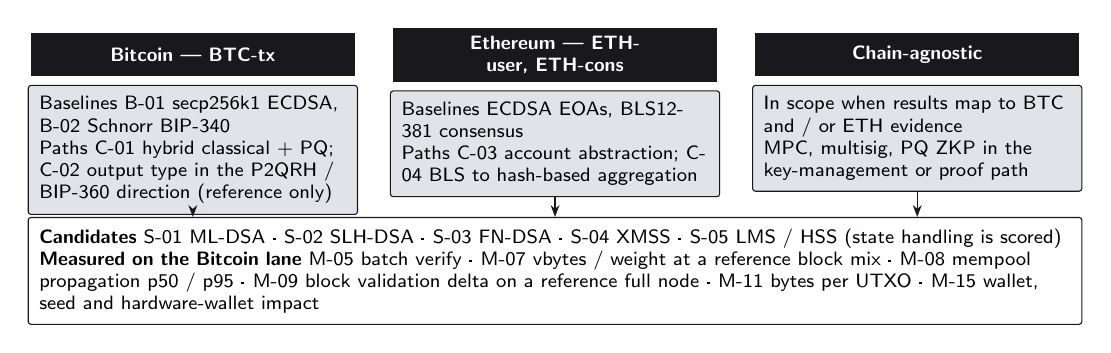
\begin{tikzpicture}[font=\scriptsize, box/.style={draw=bar,fill=lane,rounded corners=1pt,text width=3.9cm,align=left,inner sep=4pt}, hd/.style={fill=bar,text=white,font=\scriptsize\bfseries,text width=3.9cm,align=center,inner sep=3pt,minimum height=5.5mm}]
    \node[hd] (h1) at (0,0) {Bitcoin --- BTC-tx};
    \node[hd] (h2) at (4.6,0) {Ethereum --- ETH-user, ETH-cons};
    \node[hd] (h3) at (9.2,0) {Chain-agnostic};
    \node[box,below=1mm of h1] (b1) {Baselines B-01 secp256k1 ECDSA, B-02 Schnorr BIP-340\\ Paths C-01 hybrid classical + PQ; C-02 output type in the P2QRH / BIP-360 direction (reference only)};
    \node[box,below=1mm of h2] (b2) {Baselines ECDSA EOAs, BLS12-381 consensus\\ Paths C-03 account abstraction; C-04 BLS to hash-based aggregation};
    \node[box,below=1mm of h3] (b3) {In scope when results map to BTC and / or ETH evidence\\ MPC, multisig, PQ ZKP in the key-management or proof path};
    \node[draw=bar,fill=white,rounded corners=1pt,text width=13.1cm,inner sep=4pt,align=left,below=2.5mm of b2.south,anchor=north] (ev) {\textbf{Candidates} S-01 ML-DSA \textperiodcentered{} S-02 SLH-DSA \textperiodcentered{} S-03 FN-DSA \textperiodcentered{} S-04 XMSS \textperiodcentered{} S-05 LMS / HSS (state handling is scored)\\ \textbf{Measured on the Bitcoin lane} M-05 batch verify \textperiodcentered{} M-07 vbytes / weight at a reference block mix \textperiodcentered{} M-08 mempool propagation p50 / p95 \textperiodcentered{} M-09 block validation delta on a reference full node \textperiodcentered{} M-11 bytes per UTXO \textperiodcentered{} M-15 wallet, seed and hardware-wallet impact};
    \foreach \b in {b1,b2,b3} \draw[-{Stealth[length=1.5mm]},bar] (\b.south) -- (\b.south |- ev.north);
  \end{tikzpicture}
  \end{center}
  {\small Comparative scoring is anchored on Bitcoin and Ethereum. Chain-agnostic work is welcome when it can be mapped to those targets.}
  \takeaway{Japan funds the prize. BGIN turns shared evidence into standards-ready artifacts. NIST remains the reference for which PQC primitives are in scope.}
\end{frame}

% ---------------------------------------------------------------- 10 timeline (drawn)
\begin{frame}{From This Room to the 2028 Award}
  \begin{center}
  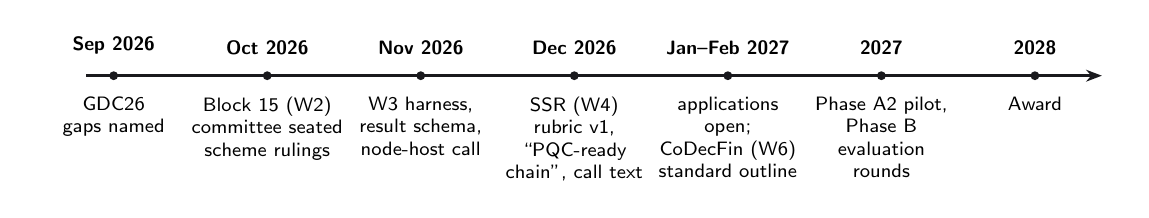
\begin{tikzpicture}[font=\scriptsize]
    \draw[line width=1pt,bar,-{Stealth[length=2mm]}] (0,0) -- (12.9,0);
    \foreach \x/\lab/\txt in {
      0.35/Sep 2026/{GDC26\\ gaps named},
      2.3/Oct 2026/{Block 15 (W2)\\ committee seated\\ scheme rulings},
      4.25/Nov 2026/{W3 harness,\\ result schema,\\ node-host call},
      6.2/Dec 2026/{SSR (W4)\\ rubric v1, ``PQC-ready\\ chain'', call text},
      8.15/Jan--Feb 2027/{applications open;\\ CoDecFin (W6)\\ standard outline},
      10.1/2027/{Phase A2 pilot,\\ Phase B evaluation\\ rounds},
      12.05/2028/{Award}}
      {\fill[bar] (\x,0) circle (1.6pt);
       \node[above=1.5mm,align=center,font=\scriptsize\bfseries] at (\x,0) {\lab};
       \node[below=1.5mm,align=center,text width=1.95cm] at (\x,0) {\txt};}
  \end{tikzpicture}
  \end{center}
  \par\vspace{1mm}
  \begin{center}\small
    Competition / evaluation $\rightarrow$ BGIN Standard $\rightarrow$ ISO/TC 307 $\rightarrow$ Japan's crypto-asset security criteria
  \end{center}
  {\scriptsize\color{soft} Dates are indicative until the host confirms the call. Bitcoin Core is not a party to any step; Bitcoin evidence is.}
  \takeaway{This conversation can still change what the call asks teams to prove. Block \#15 is the next drafting stop.}
\end{frame}

% ---------------------------------------------------------------- 11 what for
\begin{frame}{What This Session Is For}
  \begin{itemize}\small
    \item Document Bitcoin-specific \textbf{deployment gaps} --- activation, wallets and signing devices, Lightning / L2, exposed-key coins, evidence --- rather than re-litigating NIST selections.
    \item Put \textbf{resource estimates} and \textbf{migration design} in the same conversation, so urgency is argued from assumptions, not from slogans.
    \item Name where \textbf{post-quantum ZKP} and \textbf{MPC} change the key-management and proof path, without turning the hour into a ZKP-only session.
    \item Align what Bitcoin Core reviewers, wallet vendors, custodians, miners and evaluation communities each need to see before they can act --- and what stays outside Bitcoin Core's remit.
  \end{itemize}
  \takeaway{The outcome is a short list of gaps and what the metric register must measure to be useful to a Core reviewer --- not a BIP tonight.}
\end{frame}

% ---------------------------------------------------------------- 12 discussion items
\begin{frame}{Discussion Items for This Room}
  \begin{enumerate}\small
    \item Which objects move first: exposed-key UTXOs (P2PK, reused addresses), on-spend paths, Lightning channel keys, or the proof and key-management path (PQ ZKP, MPC)?
    \item What would make a \textbf{resource estimate} usable for a Bitcoin reviewer --- assumptions, error bars, and what must not be collapsed into a Q-day date?
    \item What must a \textbf{neutral testbed} measure so that ``PQ-ready'' is comparable across output types --- vbytes and weight per block, validation time on a reference full node, UTXO growth, hardware-wallet compatibility?
    \item How should \textbf{crypto agility} be specified so wallets and signing devices can rotate algorithms without a fork-by-fork rewrite --- and which of those decisions belong to Bitcoin Core at all?
  \end{enumerate}
\end{frame}

% ---------------------------------------------------------------- 13 discussion starter title
{\setbeamertemplate{footline}{}
\begin{frame}[plain,t]
  \begin{tikzpicture}[remember picture,overlay]
    \fill[bar] (current page.north west) rectangle ([yshift=-3.1cm]current page.north east);
    \node[anchor=north east,inner sep=0] at ([xshift=-7mm,yshift=-5mm]current page.north east){
\includegraphics[height=1.9cm]{bgin_logo.png}};
    \node[anchor=west,text=white,font=\Large\bfseries] at ([xshift=7mm,yshift=-1.55cm]current page.north west){Why a TLS Playbook Will Not Migrate This Stack};
    \node[anchor=west,text=white,font=\small,text width=11.2cm,align=left] at ([xshift=7mm,yshift=-2.35cm]current page.north west){A working frame for Bitcoin};
    \node[anchor=west,font=\normalsize] at ([xshift=7mm,yshift=-4.5cm]current page.north west){Shin'ichiro Matsuo, Ph.D.};
    \node[anchor=west,font=\small,text=soft] at ([xshift=7mm,yshift=-5.15cm]current page.north west){BGIN Co-Chair \textbar{} Breakout: PQC Migration on DLTs};
    \node[anchor=west,font=\small,text=soft] at ([xshift=7mm,yshift=-5.65cm]current page.north west){Global Digital Collaboration \textbar{} Geneva \textbar{} 2--3 September 2026};
    \node[anchor=west,font=\scriptsize,text=soft] at ([xshift=7mm,yshift=-6.5cm]current page.north west){Discussion starter};
  \end{tikzpicture}
\end{frame}}

% ---------------------------------------------------------------- 14 writing problem
\begin{frame}{The writing problem is not a missing algorithm}
  \lead{NIST already standardized the first primitives. Adjacent Internet protocols already have hybrid patterns. The BGIN job is not a rival scheme.}
  {\small For Bitcoin, migrating in a way that the community can actually run is hard for three stacked reasons:}\par\vspace{1.5mm}
  \pillar{0.31\textwidth}{Public verification}{Keys sit in the clear in P2PK outputs, reused addresses and every spend. Harvest-now is not only an archival problem.}\hfill
  \pillar{0.31\textwidth}{Consensus freeze}{Script validity rules are global. You cannot negotiate a cipher suite per connection the way TLS does; a new output type needs activation.}\hfill
  \pillar{0.31\textwidth}{Economic incentives}{Dormant coins, wallet UX, miner and custodian costs, and multiple implementations decide whether a clean design ships.}
  \takeaway{Design for the next migration now. A rushed cutover creates new incidents; a frozen profile goes stale.}
\end{frame}

% ---------------------------------------------------------------- 15 at-rest vs on-spend
\begin{frame}{At-Rest versus On-Spend --- Timing Is Not One Number}
  \lead{Shor recovers signing keys from exposed public keys. When the public key appears on-chain changes when the attack becomes live.}
  \pillar{0.48\textwidth}{At-rest}{The public key is already on-chain --- P2PK, a reused address, a revealed key. An adversary can grind offline against a stored verification key until a cryptographically relevant quantum computer can forge spends.}\hfill
  \pillar{0.48\textwidth}{On-spend}{The public key is revealed only when funds move. The race is then between the legitimate owner and an attacker who sees the broadcast, not an unbounded offline grind --- confirmation time is the window.}
  \par\vspace{1.5mm}
  {\small Address design, reuse, and wallet defaults therefore change the threat model (the PRX Quantum taxonomy adds a third case, \emph{on-setup}, for keys exposed during multi-party setup). A single Q-day slogan erases that difference.}
  \takeaway{Resource estimates only become policy-useful when they are tied to which keys are already public.}
\end{frame}

% ---------------------------------------------------------------- 16 questions
\begin{frame}{Questions for this room}
  \lead{This session is for mapping gaps and naming what Block \#15 must decide --- not for locking a first migration spec tonight.}
  \begin{enumerate}\small
    \item Which \textbf{objects} should be triaged first, and which can wait: at-rest keys, on-spend paths, Lightning channels, PQ ZKP, MPC?
    \item What would make a \textbf{resource estimate} honest enough for this audience --- and what language should we refuse (single Q-day, vendor screenshots)?
    \item What must a \textbf{neutral evaluation} see so that hybrid then cutover is comparable across Bitcoin-class, account-model, and wallet stacks?
    \item How should agility be written so wallet and signing-device profiles can \textbf{rotate} without forking the scheme every time the primitive list moves?
  \end{enumerate}
\end{frame}

% ---------------------------------------------------------------- 17 join
\begin{frame}{Join us at BGIN Block 15}
  \lead{15--16 October 2026 \textbar{} Georgetown University Capitol Campus, 111 Massachusetts Ave NW, Washington, D.C. \textbar{} In person (remote available). The PQC drafting and measurement work above continues in the Block 15 IKP sessions.}\vspace{-1.5mm}
  {\small\textbf{Related sessions}}
  \begin{itemize}\small
    \item 15 Oct, 09:20--09:50 (Room A). Keynote: PQC
    \item 15 Oct, 09:50--11:20 (Room B). IKP: PQC Migration (1) --- resource estimates into judging criteria
    \item 15 Oct, 11:30--13:00 (Room B). IKP: PQC Migration (2) --- crypto agility as governance; NIST migration path
  \end{itemize}
  \par\vspace{-1mm}
  \begin{center}\tiny
    \begin{tabular}{@{}>{\centering\arraybackslash}p{3.1cm}@{\hspace{2mm}}>{\centering\arraybackslash}p{3.1cm}@{\hspace{2mm}}>{\centering\arraybackslash}p{3.1cm}@{\hspace{2mm}}>{\centering\arraybackslash}p{3.1cm}@{}}
      \qrcode[height=1.25cm]{https://bgin-global.org/events/20261015-block15/sessions/1-4} &
      \qrcode[height=1.25cm]{https://bgin-global.org/events/20261015-block15} &
      \qrcode[height=1.25cm]{https://www.eventbrite.com/e/bgin-block15-tickets-1990274282957} &
      \qrcode[height=1.25cm]{https://github.com/bgin-global/pqc-agility-competition} \\[0.5mm]
      \textbf{PQC session} & \textbf{Block 15 site} & \textbf{Register} & \textbf{Competition repo} \\
      bgin-global.org/events/ 20261015-block15/sessions/1-4 & bgin-global.org/events/ 20261015-block15 & eventbrite.com/e/ bgin-block15-tickets & github.com/bgin-global/ pqc-agility-competition
    \end{tabular}
  \end{center}
  \takeaway{Hybrid. Connection details are sent after registration; fee waivers for written contributions. You are invited.}
\end{frame}

\end{document}
